\chapter{Background}

\section{Introduzione al DNS e al filtraggio}
Prima di trattare l'argomento cardine del presente capitolo, si ritiene opportuno fare una breve panoramica sui concetti importanti ad esso collegati. Verrà in prima batttuta presentato il Domain Name System (DNS), che può essere definito come uno dei pilastri fondamentali di tutta l'architettura della rete Internet. Successivamente, ci si sposterà sull'ambito del filtraggio in Internet, che rappresenta il contesto più ampio di cui il filtraggio DNS fa parte.

\subsection{Cos'è il DNS e il suo ruolo in Internet}
Il Domain Name System è un database gerarchico e distribuito che contiene le associazioni tra nomi di dominio ed altre importanti informazioni, tra cui gli indirizzi IP.

Questo fondamentale sistema consente agli utenti di localizzare le risorse sulla rete andando a convertire nomi di dominio familiari ed in formato leggibile dagli umani in indirizzi numerici ai quali un computer può connettersi. Un'analogia comune che si uutilizza per spiegare il ruolo dei sistema DNS è che esso serve da rubrica telefonica per Internet, andando a tradurre i nomi di computer comprensibili agli umani nei relativi indirizzi numerici interpretabili dalle macchine. Per fare un esempio, il nome di dominio \texttt{www.airbus.com} viene tradotto dal DNS nell'indirizzo IPv4 \texttt{107.154.76.155}.

\subsubsection{Vulnerabilità del DNS}
Il DNS rappresenta una porzione cruciale della rete Internet e per questo motivo la sua messa in sicurezza risulta molto importante. Infatti, se un individuo malintenzionato dovesse riuscire a comprometterlo, sarebbe in grado di bloccare, o comunque ridurre, le normali attività che avvengono sulla rete.

Il sistema in oggetto è stato progettato negli anni '80 per rispondere alla necessità di una risoluzione dei nomi rapida e scalabile su una rete in continua espansione. Al momento della sua concezione, come descritto nelle specifiche originarie RFC 1034 \cite{rfc1034} e RFC 1035 \cite{rfc1035}, l'attenzione era principalmente concentrata sulla funzionalità e sull'efficienza, senza considerare i potenziali problemi di sicurezza che sarebbero emersi con la crescita esponenziale di Internet. Oltretutto, la solida fiducia che le specifiche RFC trasmettevano ai professionisti IT dell’epoca non li spinse a preoccuparsi o a indagare sui potenziali rischi di sicurezza che tale sistema poteva comportare \cite{hudaib2014dns}. Questa scelta rifletteva il contesto storico in cui è nato il DNS: la rete era allora utilizzata principalmente da enti accademici e governativi, con un livello di fiducia reciproca tra i partecipanti. Tuttavia, con l'apertura di Internet a un pubblico globale, il DNS ha rivelato vulnerabilità intrinseche, tra cui la mancanza di meccanismi nativi che garantiscano l'autenticazione delle risposte e l'integrità delle informazioni da esso fornite. Tali lacune hanno reso possibile una serie di attacchi che sfruttano le debolezze proprie del sistema DNS. Tra questi, si annoverano il DNS Spoofing, gli attacchi di tipo Distributed Denial of Service (DDoS) nei confronti dell'infrastruttura DNS e il DNS Hijacking.

\paragraph{DNS Spoofing}
Il DNS spoofing, noto anche come Cache Poisoning, consiste nell'iniettare dati malevoli nella cache dei server DNS bersaglio, inducendoli a restituire informazioni errate agli utenti. Questo attacco permette ai malintenzionati di reindirizzare il traffico verso siti controllati da essi, facilitando il furto di credenziali o altre forme di attacchi avanzati. Un esempio storico di DNS spoofing è l'attacco di Eugene Kashpureff del 1997, il quale riuscì a reindirizzare tutti i visitatori del dominio \texttt{internic.net} verso il sito della compagnia Alternic, di cui era il fondatore \cite{lioy2000dns}. In generale, questa tipologia di attacco sfrutta la mancanza di autenticazione nelle risposte DNS e l'assenza di integrità nelle informazioni memorizzate nella cache. I metodi per mitigare il DNS spoofing includono sostanzialmente l'implementazione di DNSSEC, che garantisce l'autenticità delle risposte attraverso firme digitali \cite{rfc2535}.

\paragraph{Attacchi di amplificazione DNS}
Gli attacchi Distributed Denial of Service (DDoS) rappresentano una minaccia critica e persistente per la sicurezza informatica. In generale, essi mirano a compromettere la disponibilità dei servizi di un sistema bersaglio, costringendolo a un riavvio forzato o esaurendone le risorse, come cicli della CPU, memoria RAM o larghezza di banda di rete. A conseguenza di ciò, il sistema attaccato diventa incapace di fornire i servizi previsti agli utenti legittimi.

Tra le più comuni applicazioni del DDoS nei confronti dell'infrastruttura DNS è possibile trovare i cosiddetti DNS Amplification Attacks, in cui un attaccante invia richieste al Domain Name System con un indirizzo IP sorgente falsificato, facendole apparire come provenienti dalla vittima. A questo punto, i server DNS rispondono con pacchetti di dimensioni molto superiori rispetto alla richiesta iniziale, amplificando così il traffico diretto alla vittima.
%
Il principio alla base di questa tecnica risiede nella capacità degli attaccanti di sfruttare la differenza tra la dimensione delle richieste e quella delle risposte. Ad esempio, una richiesta per un grande file di zona DNS, con l'indirizzo IP sorgente falsificato, viene inviata a un numero significativo di server DNS pubblici. Questi, ignari della natura fraudolenta delle richieste, rispondono inviando i dati direttamente alla vittima designata. La differenza di dimensioni tra la richiesta, tipicamente piccola, e la risposta, significativamente più grande, permette agli attaccanti di moltiplicare il volume di traffico generato, compromettendo gravemente il sistema bersaglio \cite{Alieyan2016}.

Un esempio di amplificazione DNS è quello che ha colpito Spamhaus nel 2013, considerato uno dei più grandi attacchi DDoS mai accaduti. Esso è stato caratterizzato da una richiesta di 36 byte che ha generato una risposta di 3.000 byte, amplificando il traffico di un fattore 100 e generando un volume di dati in entrata ai server della compagnia pari a 75GBps \cite{Bonasera2021}.

\paragraph{DNS Hijacking}
Il DNS hijacking prevede la compromissione di server DNS o la manipolazione delle configurazioni DNS di un utente per reindirizzare il traffico verso destinazioni controllate da un malintenzionato. Questo tipo di attacco può essere implementato seguendo due strategie \cite{hudaib2014dns}:
\begin{itemize}
  \item attraverso l'uso di specifici malware che modificano le impostazioni DNS locali
  \item mediante la compromissione diretta dei server DNS fidati, in modo che non si comportino come da specifica.
\end{itemize}

Le conseguenze includono il furto di credenziali, la diffusione di malware e la censura di contenuti web. Tuttavia, alcuni provider di servizi Internet (ISP) utilizzano questa tecnica per scopi commerciali, come la visualizzazione di pubblicità o la raccolta di statistiche sulla avigazione dei propri utenti. Per mitigare il DNS hijacking, si consiglia di utilizzare configurazioni DNS sicure e controllare in maniera scrupolosa le modifiche ai record DNS locali \cite{hudaib2014dns}.

\subsection{Il filtraggio di Internet}
A seguito dell'analisi riguardante le vulnerabilità intrinseche del sistema DNS, emerge chiaramente l'importanza di adottare meccanismi di prevenzione per garantire una navigazione più sicura e controllata. A questo proposito, una soluzione interessante riguarda il filtraggio di Internet, che, in generale, rappresenta un insieme di tecniche e tecnologie volte a limitare o bloccare l'accesso a contenuti considerati inappropriati, illegali o dannosi. Le principali pratiche di filtraggio nell'ambito di Internet si dividono nelle tre seguenti tipologie:
\begin{itemize}
  \item \textbf{IP Packet Filtering}: ovvero il blocco del traffico basato su indirizzi IP o numeri di porta. Questa tecnica analizza gli header dei pacchetti per decidere se consentirne il passaggio o eliminarli. Sebbene sia semplice ed efficiente, può causare sovrafiltraggio, rendendo inaccessibili quei contenuti legittimi ospitati sullo stesso IP considerato malevolo;

  \item \textbf{DNS Poisoning}: consiste nella manipolazione delle risposte DNS per reindirizzare richieste a indirizzi errati o per bloccarle completamente. Sebbene sia nata come una pratica malevola, i suoi principi tecnici sono stati adattati ed applicati ad un contesto legittimo di filtraggio;

  \item \textbf{URL Blocking}: implementa il blocco di URL specifici tramite proxy HTTP o tecniche come la Deep Packet Inspection (DPI). Questi sistemi analizzano il contenuto delle richieste HTTP per identificare e bloccare pagine o risorse specifiche, offrendo una maggiore precisione rispetto ai metodi sopra elencati. L'unico svantaggio di quest'ultimo approccio deriva dal fatto che risulta più complesse da implementare e richiede maggiori risorse rispetto alle altre tecniche.
\end{itemize}

\subsubsection{Punti di applicazione del filtraggio di Internet}
Il filtraggio di Internet può essere implementato in diversi livelli dell'architettura di rete, con implicazioni specifiche in termini di efficacia, costi e complessità. Secondo V. Varadharajan \cite{Varadharajan2010}, i principali punti di applicazione includono:

\begin{itemize}
  \item \textbf{A monte dell'ISP}: i filtri possono essere posizionati nei fornitori internazionali di connettività o presso le dorsali di rete. Questo approccio consente di bloccare contenuti indesiderati prima che raggiungano l'ISP locale, risultando particolarmente utile per gestire traffico proveniente da server internazionali. Tuttavia, questa strategia richiede una stretta collaborazione tra le entità coinvolte e una chiara mappatura dei gateway internazionali.

  \item \textbf{All'interno dell'ISP}: posizionare i filtri nel core della rete ISP permette di monitorare e controllare il traffico a livello centralizzato per tutti gli utenti dell'ISP. Sebbene sia efficace, questa soluzione può introdurre colli di bottiglia e richiedere investimenti significativi in hardware sofisticato, soprattutto per ISP con un alto volume di traffico.

  \item \textbf{Tra l'ISP e il cliente}: applicare il filtraggio nel collegamento tra l'ISP e il cliente finale offre un controllo mirato sul traffico diretto verso reti locali o singoli utenti. Questa configurazione consente di personalizzare le policy di filtraggio, ma può comportare costi operativi elevati per ISP con grandi numeri di clienti.

  \item \textbf{Tra due clienti dello stesso ISP}: in reti locali o interne a un ISP, i filtri possono essere configurati per impedire lo scambio di contenuti indesiderati tra utenti dello stesso provider. Questo approccio è utile in contesti aziendali o comunità chiuse.

  \item \textbf{Tra un cliente e un sito web ospitato a livello internazionale}: i filtri possono essere utilizzati per monitorare e bloccare il traffico tra un utente e server internazionali. Questa strategia è cruciale per controllare contenuti provenienti dall'estero ma richiede la capacità di gestire connessioni transfrontaliere e un'infrastruttura adeguata.
\end{itemize}

La caratteristica delle tecniche di filtraggio che consente loro di essere distribuite su diversi livelli, fornisce un'elevata flessibilità nell'implementazione delle strategie di controllo dei contenuti.
Tuttavia, ogni livello si porta con sé alcuni compromessi: il posizionamento a monte può bloccare grandi volumi di traffico, ma con rischi di sovrafiltraggio, mentre i filtri localizzati vicino agli utenti offrono maggiore precisione ma richiedono risorse significative. Una combinazione di approcci, come quella messa in atto dalla British Telecom’s CleanFeed, può ottimizzare l'efficacia del filtraggio, bilanciando precisione e scalabilità \cite{Varadharajan2010}.

\subsection{Il filtraggio DNS}
Tra le varie tecniche di Internet filtering descritte in precedenza, il filtraggio a livello DNS si distingue per la sua semplicità e versatilità. Al contrario di altri approcci, esso agisce direttamente sul sistema che costituisce la base della navigazione online. Questo lo rende un punto di controllo strategico ed efficace per implementare politiche di sicurezza e controllo dell'accesso. Oltretutto, i cybercriminali stanno sempre di più prendendo di mira il DNS per condurre le loro attività malevole. Per questo motivo, le tecniche di filtraggio a questo livello risultano ancora più centrali nella missione di rendere la rete più sicura e gli utenti meno a rischio di essere colpiti da attacchi.

Nei paragrafi che seguono, verrà proposta una definizione della tecnica in oggetto, fornendo anche alcuni dettagli sulle sue possibili applicazioni pratiche e sulle tecniche che ne abilitano il funzionamento.

Il \textit{DNS Filtering} consiste nell'applicare regole predefinite per bloccare o consentire richieste e risposte DNS, analogamente a quello che fa un firewall. Questa tecnica è in grado di prevenire l'accesso a contenuti malevoli o inappropriati, supportare l'applicazione di politiche aziendali e proteggere gli utenti da minacce provenienti dalla rete \cite{Magnusson2024}. Volendo essere più specifici, il filtraggio DNS trova applicazione in una vasta gamma di scenari pratici \cite{Murdoch2008, Varadharajan2010}:
\begin{itemize}
  \item \textbf{Sicurezza informatica}: viene utilizzato per bloccare siti di phishing o che distribuiscono malware e altri contenuti dannosi;

  \item \textbf{Applicazione di politiche aziendali}: permette alle organizzazioni di imporre restrizioni sull'accesso a siti non correlati al lavoro, come social media o piattaforme di streaming, durante l'orario lavorativo;

  \item \textbf{Controllo parentale}: consente la creazione di un ambiente sicuro per i minori, limitando l'accesso a contenuti non appropriati come siti per adulti o violenti;

  \item \textbf{Gestione della larghezza di banda}: aiuta a limitare l'accesso a siti che consumano molta banda, come i servizi di streaming video, ottimizzando così l'utilizzo delle risorse di rete.
\end{itemize}

Dopo aver introdotto il concetto di filtraggio DNS e averne illustrato le principali applicazioni pratiche, è importante approfondire le tecniche utilizzate per la sua implementazione. Sebbene il \textit{DNS Filtering} sia ampiamente riconosciuto come uno strumento fondamentale per migliorare la sicurezza delle reti, la sua efficacia dipende dall'applicazione di metodi avanzati per identificare e bloccare le minacce. Come evidenziato in letteratura, la ricerca ha individuato tre tecniche principali che rappresentano lo stato dell'arte in questo campo: le \textit{Response Policy Zones} (RPZ), i \textit{Threat Intelligence Feeds} (TIF) e il rilevamento di domini generati algoritmicamente (\textit{Domain Generation Algorithm}, DGA) \cite{Magnusson2024}.

Queste tecniche non solo permettono di affrontare le minacce più comuni, come phishing e malware, ma forniscono anche strumenti per rispondere a sfide più complesse, come il rilevamento di domini dinamici utilizzati dalle botnet. Tuttavia, la letteratura sottolinea anche alcune lacune, in particolare la mancanza di un'analisi integrata di queste metodologie. Approfondire ciascuna di esse consente di comprendere meglio il loro funzionamento, le applicazioni e i limiti, fornendo una base solida per ulteriori miglioramenti nel campo del DNS Filtering. A questo proposito, le sezioni seguenti saranno dedicate all'approfondimento delle tecniche appena citate, per poi fornire uno spunto su come potrebbero essere unite insieme per migliorare significativamente le performance del filtri.

\subsubsection{Response Policy Zones}
L'espressione Response Policy Zones descrive una funzionalità dei resolver DNS che consente agli amminsitratori di rete di specificare politiche per le risposte DNS, sulla base dei nomi di dominio e del contesto. Questa tecnologia di firewall DNS basata sulla reputazione opera intercettando le query e le risposte DNS, e poi le confronta con un elenco di politiche definite dall'amministratore. Quando viene rilevata una corrispondenza, il resolver restituisce una risposta in base alla politica, che poi rappresenta l'azione da compiere. Esempi di possibili azioni, sono bloccare una certa query oppure reindirizzarla verso un sito sicuro (si veda la figura \Cref{fig:rpz}).

\begin{figure}
  \centering
  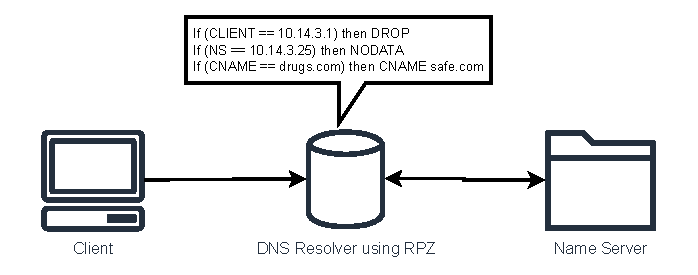
\includegraphics[width=1.0\linewidth]{figures/Response_Policy_zones.pdf}
  \caption{Un resolver DNS che sfrutta le Response Policy Zones}
  \label{fig:rpz}
\end{figure}

Le RPZ rappresentano un potente strumento per l'applicazione delle politiche di sicurezza e per proteggere la rete da attività malevole. Inoltre, il loro essere flessibili e personalizzabili, consente agli amministratori di definire policy molto specifiche, che si addatano a qualsiasi necessità. Tuttavia, per evitare falsi positivi e per mantenere l'efficacia del sistema nel tempo, le RPZ necessitano di una corretta configurazione e manutenzione. Infatti, le policy hanno costantemente bisogno di essere mantenute aggiornate, partendo da informazioni accurate ed affidabili.

Infine, si ritiene opportuno puntualizzare un limite di questa tecnologia. In particolare, le RPZ sono in grado di proteggere solamente da minaccie conosciute. Ciò deriva dalla natura stessa di questa tecnica di filtraggio, che fa affidamento su delle policy definite sulla base di minaccie necessariamente già inquadrate e studiate.

\subsubsection{Threat Intelligence Feeds}
Prima di descrivere la tecnica di filtraggio in sé, si ritiene necessario presentare brevemente i concetti ad essa associati: l'espressione \textit{cyber threat intelligence} si riferisce ad un insieme di informazioni relative a minacce informatiche potenziali o reali, utili per migliorare la situazione di una organizzazione in termini di sicurezza.
%
Queste informazioni possono includere dettagli su tattiche, tecniche e procedure (TTP) adottate da attori malevoli noti, nonché indicatori di compromissione (IOC) come indirizzi IP, nomi di dominio e hash di malware. Nel contesto del DNS, i Threat Intelligence Feeds costituiscono dati aggiornati sui domini malevoli e relativi indirizzi IP.

I TIF possono provenire da fonti diverse, tra cui intelligence open-source, fornitori commerciali e gruppi di condivisione delle minacce specifici per settore. Questi flussi includono elenchi di IOC generati analizzando il traffico di rete, i log di sicurezza o altre fonti di intelligence. I resolver, quindi, possono utilizzare questi dati per bloccare o reindirizzare le query DNS verso domini malevoli noti.

In generale, l'integrazione dei TIF nel filtraggio DNS offre una difesa efficace contro le minacce conosciute e aiuta le organizzazioni a rilevare e prevenire gli attacchi prima che possano causare danni. Tuttavia, è importante ricordare che i flussi in questione non rappresentano una soluzione definitiva e devono essere utilizzati insieme ad altre misure di sicurezza per garantire una protezione completa.

\subsubsection{Domain Generation Algorithms}
Rappresenta una metodologia che attuanoo i malware per la generazione di nomi di dominio univoci, volti a consentire la comunicazione tra le vittime ed i server \textit{Command-and-Control} (C2). Tali domini, vengono solitamente generati partendo dalla data e ora corrente, rendendo il processo di blocco molto difficile da parte dei sistemi di filtraggio che si basano su liste statiche di indirizzi IP malevoli. Però, sfruttando specifici algoritmi di Machine Learning, è possibile rilevare questi domini casuali, cercando di riconoscere dei pattern che caratterizzano i domini generati algoritmicamente. Più in dettaglio, se si analizza la struttura dei nomi di dominio prodotti dai malware, insieme al comportamento ed al contesto delle query DNS, è possibile rilevare e quindi bloccare le comunicazioni con i server C2, anche se i domini malevoli compaiono una sola volta.

\subsubsection{Uso combinato di RPZ, TIF e rilevamento DGA}
L'uso combinato di Response Policy Zones (RPZ), Threat Intelligence Feeds (TIF) e tecniche di rilevamento di algoritmi di generazione di domini (DGA) rappresenta un approccio promettente per migliorare l'efficacia del filtraggio DNS. Le RPZ possono intercettare le query DNS, confrontandole con blocklist e allowlist, mantenute costantemente aggiornate grazie ai TIF. A loro volta, i TIF possono integrare tecniche avanzate di rilevamento DGA per identificare domini malevoli conosciuti e sconosciuti, analizzando query anonimizzate.

Un framework che integri queste tecniche può migliorare notevolmente la capacità di rilevare e bloccare domini malevoli, minimizzando i falsi positivi e garantendo un'intelligence tempestiva e accurata. La trasparenza nel processo di filtraggio, che si concretizza nel remdere pubblicamente disponibili le liste di filtri, può favorire la fiducia degli utenti e prevenire abusi come la censura. Inoltre, il coinvolgimento della community attraverso contributi di esperti e ricercatori nell'ambito della sicureza informatica, può ulteriormente rafforzare l'efficacia del sistema.

Se da un lato ci sono dei vantaggi nel rendere pubbliche tali informazioni, dall'altro potrebbero emergere argomentazioni a sfavore di questa attività. Infatti, i malintenzionati sarebbero in grado di adattare le loro metofologie di attacco sulla base delle consultabili politiche di filtraggio. Ciononostante, questo approccio potrebbe generare dei vantaggi indiretti, derianti dal fatto che i creatori di malware sarebbero costretti a modificare i propri metodi di attacco, rendendo il loro comportamento più visibile all'interno del traffico di rete. Questo fatto faciliterebbe l'itendificazione e lo studio di nuove tecniche di. Questo cambiamento, a sua volta, puù aiutare i ricercatori, e in generale i difensori, a venrie a conoscenza delle nuove tecniche di evasione emsse in campo dai cybercriminali \cite{Magnusson2024}.

\section{Metodologie di reingegnerizzazione software}

\subsection{Introduzione alla Reingegnerizzazione}

\subsection{Fasi del Processo di Reingegnerizzazione}
